% !TEX root = ./MATH2160.tex
\chapter{Fundamentals}\label{chapter:Fundamentals}

Numerical analysis is the design and analysis of accurate and efficient algorithms to solve problems in science and engineering. Computers work with numbers which can be represented by finitely many bits, whereas some real numbers require infinitely many bits to represent exactly. Thus, there is an error involved in representing each real number, and this error propagates in subsequent arithmetic operations. An analysis is required to determine in which instances we can trust the result of a long sequence of calculations and in which instances we should design a better algorithm or use higher precision.

Standard domains used in these notes include the natural numbers $\N$, the integers $\Z$, the rationals $\Q$, and:
\begin{center}
\begin{tabular}{cccccc}
\sphline
Name & Unit Interval & Real Line & Complex Plane & Torus & Unit Circle\\
\sphline
Notation & $\I$ & $\R$ & $\C$ & $\T$ & $\U$\\
\sphline
Definition & $[-1,1]$ & $(-\infty,+\infty)$ & $\{z = x+\i y : x,y\in\R\qand \i^2=-1\}$ & $[0,2\pi)$ & $e^{\i\T}$\\
\sphline
\end{tabular}
\end{center}%

\section{Vector Spaces}

\begin{definition}\label{definition:vectorspace}
A set $V$ with elements from the field $\F$, together with operations of vector addition and scalar multiplication, is a {\em vector space} if it satisfies the following axioms. For all vectors $u,v,w\in V$ and for all scalars $\alpha,\beta\in\F$:
\begin{enumerate}
\item Associativity of Addition: $u+(v+w) = (u+v)+w$;
\item Commutativity of Addition: $u+v = v+u$;
\item Identity Element of Addition: $\exists 0\in V: u+0 = u$;
\item Inverse Elements of Addition: $\exists -v\in V: v+(-v) = 0$;
\item Compatibility of Scalar Multiplication: $\alpha(\beta v) = (\alpha\beta)v$;
\item Identity Element of Scalar Multiplication: $1v = v$;
\item Distributivity of Scalar Multiplication with Respect to Vector Addition: $\alpha(u+v) = \alpha u + \alpha v$; and,
\item Distributivity of Scalar Multiplication with Respect to Scalar Addition: $(\alpha + \beta)u = \alpha u + \beta u$.
\end{enumerate}
\end{definition}

\begin{example}
Let $n\in\N$. The spaces $\R^n$ and $\C^n$ are vector spaces. However, the space $\R_{\ge0} = \{x\in\R:x\ge0\}$ is not a vector space because inverse elements of addition are absent.
\end{example}

\begin{example}
The set of functions from any fixed set $D$ to elements in the field $\F$ forms a vector space since for any $x\in D$ and $\alpha\in\F$:
\[
(f+g)(x) = f(x) + g(x),\quad{\rm and}\quad (\alpha f)(x) = \alpha f(x).
\]
\end{example}

\subsection{Normed Vector Spaces}

The essential notions of size and distance in a vector space are captured by norms. These are the yardsticks with which we measure approximations and convergence throughout numerical analysis.

\begin{definition}\label{definition:norm}
A {\em norm} is a function $\|\cdot\|:V\to\R$ that assigns a real-valued length to each vector. In order to conform to a reasonable notion of length, a norm must satisfy the following three conditions. For all vectors $x$ and $y$ and for all scalars $\alpha\in\F$:
\begin{enumerate}
\item $\norm{x}\ge0$, and $\|x\| = 0$ only if $x=0$;
\item $\norm{x+y} \le \norm{x}+\norm{y}$; and,
\item $\norm{\alpha x} = \abs{\alpha}\norm{x}$.
\end{enumerate}
\end{definition}
In words, these conditions require that 1.~the norm of a nonzero vector is positive, 2.~the norm of a vector sum does not exceed the sum of the norms of its parts--the {\em triangle inequality}, and 3.~scaling a vector scales its norm by the same amount.

The most important class of vector norms, the $p$-norms, are defined below. The closed unit ball $\{x\in \C^n:\norm{x}\le1\}$ corresponding to each norm is illustrated to the right for the case $n=2$.

\begin{equation}
\begin{array}{llc}
\norm{x}_1 & = \displaystyle\sum_{i=1}^n\abs{x_i}, & 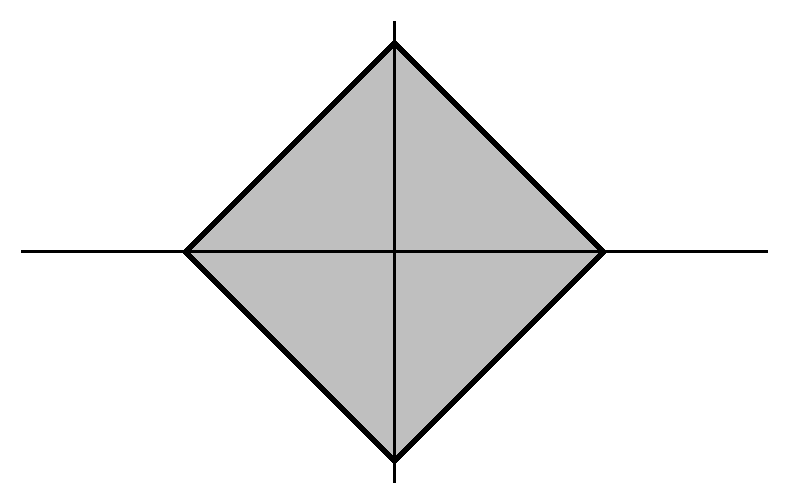
\includegraphics[width=0.15\textwidth]{norm1}\\
\norm{x}_2 & = \displaystyle\left(\sum_{i=1}^n\abs{x_i}^2\right)^{\frac{1}{2}} = \sqrt{x^*x}, & 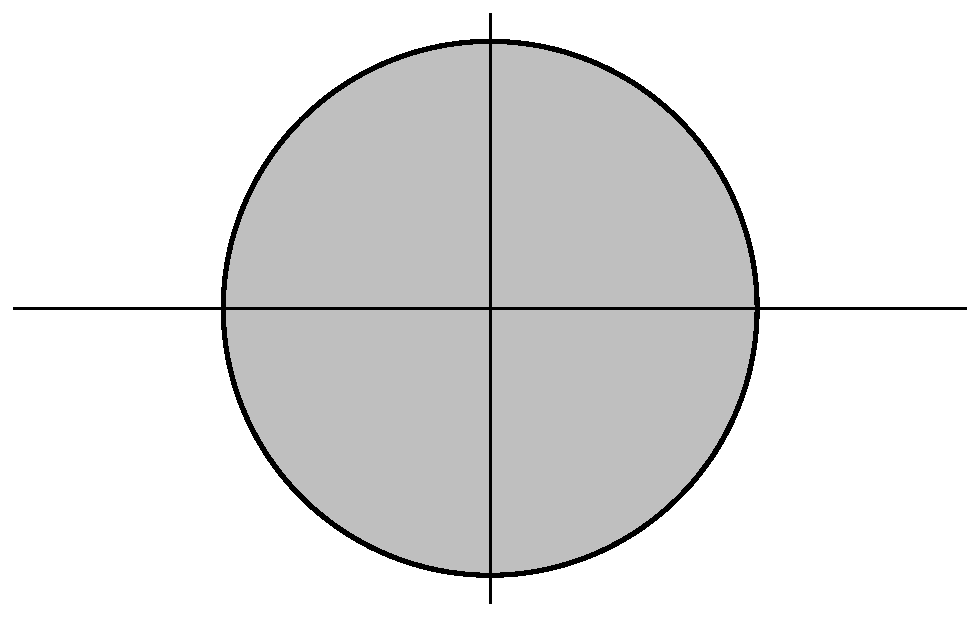
\includegraphics[width=0.15\textwidth]{norm2}\\
\norm{x}_p & = \displaystyle\left(\sum_{i=1}^n\abs{x_i}^p\right)^{\frac{1}{p}},\quad (1\le p < \infty), & 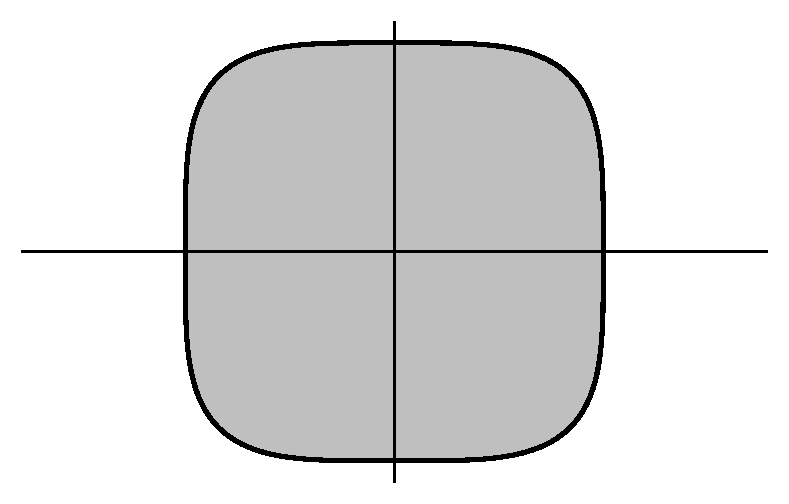
\includegraphics[width=0.15\textwidth]{norm4}\\
\norm{x}_\infty & = \displaystyle\max_{1\le i\le n}\abs{x_i}, & 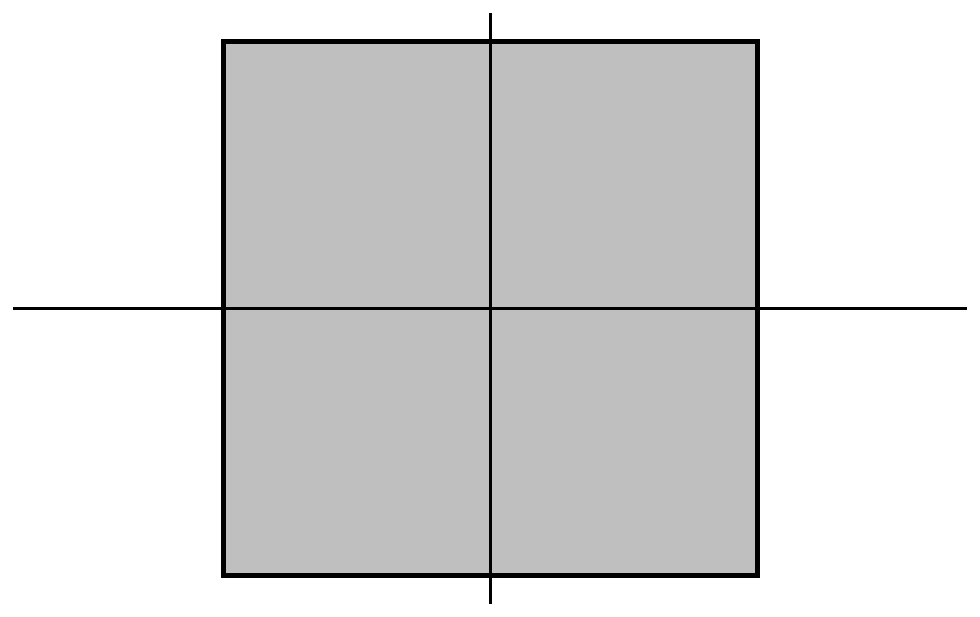
\includegraphics[width=0.15\textwidth]{norminf}\\
\end{array}
\end{equation}

The $2$-norm is the Euclidean length function; its unit ball is spherical. The $1$-norm is known as the Manhattan norm since it is the distance a taxi has to drive in a street grid\footnote{The $1$-norm is also used by airlines to define the maximal allowable size of a suitcase.}. The Sergel plaza in Stockhom, Sweden has the shape of the unit ball in the $4$-norm; the Danish poet Piet Hein popularized this ``superellipse'' as a pleasing shape for objects such as conference tables.

Aside from the $p$-norms, the most useful norms are the {\em weighted $p$-norms}, where each of the coordinates of a vector space is given its own weight. In general, given any norm $\norm{\cdot}$, a weighted norm can be written as:
\begin{equation}
\norm{x}_W = \norm{Wx}.
\end{equation}
Here, $W$ is the diagonal matrix in which the $i^{\rm th}$ diagonal entry is the weight $w_i\ne0$. For example, a weighted $2$-norm $\|\cdot\|_W$ on $\C^n$ is specified as follows:
\begin{equation}
\norm{x}_W = \left(\sum_{i=1}^n\abs{w_ix_i}^2\right)^{\frac{1}{2}}.\hspace*{2.5cm} 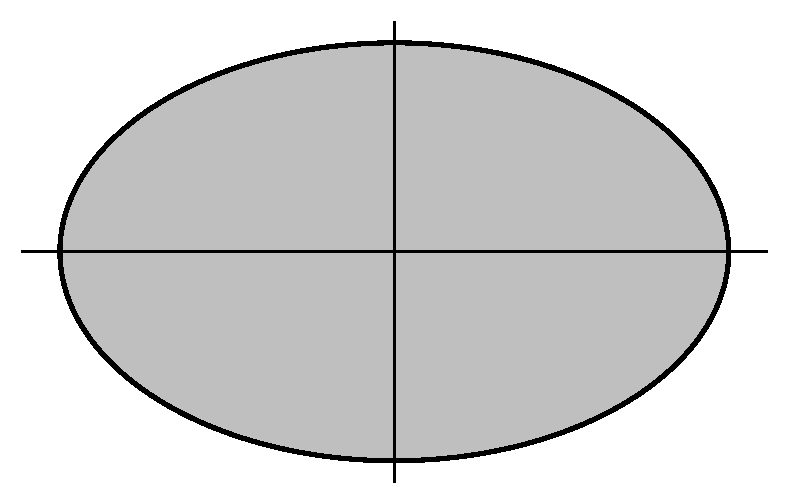
\includegraphics[width=0.15\textwidth]{normW}
\end{equation}
One can also generalize the idea of weighted norms by allowing $W$ to be an arbitrary nonsingular matrix.

The most important norms in this book are the unweighted $2$-norm and its induced matrix norm.

The concept of the $p$-norms can be extended to the case of vector spaces containing infinitely many elements. Such spaces are called sequence spaces, and the following spaces describe sequence spaces that have finite norm.

\begin{definition}
Let $1\le p\le\infty$. The space $\ell^p$ contains the set of all vectors $x\in V$ with finite $p$-norm:
\begin{equation}
\ell^p = \{ x\in V: \norm{x}_p < \infty\}.
\end{equation}
\end{definition}

\begin{example}
Every vector $x\in\R^n$ is in $\ell^p$. Consider the vector $y\in\R^\infty$ whose entries are defined by:
\begin{equation}
y_i = \dfrac{1}{i},\quad{\rm for}\quad i=1,\ldots,\infty.
\end{equation}
Then, $y\in\ell^p$ for every $p>1$ since for every $\epsilon>0$, $\sum_{i=1}^\infty i^{-1-\epsilon} < \infty$ by the integral test for convergence.
\end{example}

While we will not focus on $\ell^p$ spaces in this course, we will be interested in their analogues for functions.

\subsection{Function Spaces}

Let $D\subset\R$ or $\C$ denote the domain of a function $f$. 

\begin{definition}
A function is continuous at every point $c\in D$ if $f(c)$ exists and if $\displaystyle\lim_{\substack{x\to c \\ x \in D}}f(x) = f(c)$. \end{definition}

\begin{definition} The space:
\begin{itemize}
\item $C(D)$ contains all continuous functions on $D$;
\item $C^n(D)$ contains all functions whose $n^{\rm th}$ derivatives are continuous on $D$;
\item $C^\infty(D)$ contains all functions with continuous derivatives of all orders on $D$; and,
\item $A(D)$ contains all functions analytic on $D$. That is, they are equal to their Taylor series at every point in $D$.
\end{itemize}
\end{definition}

\begin{example}
The functions:
\begin{itemize}
\item $f(x) = \abs{x} \in C(\I)$;
\item $f(x) = \abs{x}^{n+1}\in C^n(\I)$ ($n$ even\footnote{For $n$ odd $\abs{x}^{n+1}$ is a polynomial and polynomials are entire.});
\item $f(x) = \left\{\begin{array}{ccc} e^{-1/x^2} & \for & x\ne 0,\\0 & \for & x = 0,\end{array}\right.\in C^\infty(D)$ for every $0\in D\subset\C$;
\item $f(x) = \dfrac{1}{1+x^2} \in A(D)$ where $D = \{z\in\C:\abs{z}<1\}$ is the open unit disk; and,
\item $f(x) = \sin x\in A(\C)$.
\end{itemize}
\end{example}

The analytic functions $A(\C)$ are so smooth that they are further denoted as {\em entire} functions.

The notion of a vector $p$-norm extends readily to functions that are Lebesgue integrable. For $1\le p < \infty$:
\begin{equation}
\|f\|_p := \left(\int_D\abs{f(x)}^p\ud x\right)^{\frac{1}{p}},
\end{equation}
and for $p=\infty$:
\begin{equation}
\|f\|_\infty := \sup_{x\in D} \abs{f(x)}.
\end{equation}
Sometimes the measure is not uniform. These cases correspond to the weighted $p$-norms:
\begin{equation}
\|f\|_{p,\mu} := \left(\int_D\abs{f(x)}^p\ud\mu(x)\right)^{\frac{1}{p}}.
\end{equation}

\begin{definition}
The space $L^p(D,\ud\mu(x))$ contains all functions Lebesgue\footnote{This definition ignores functions that are zero almost-everywhere, in which case the functions are indistinguishable from zero in norm since $\norm{f}_p=0$.} integrable on $D$ with respect to the measure $\ud\mu(x)$:
\begin{equation}
L^p(D,\ud\mu(x)) := \left\{ f : \norm{f}_{p,\mu} < \infty \right\}.
\end{equation}
\end{definition}

\begin{remark}
\begin{enumerate}
\item When it is clear from the context, the measure $\ud\mu(x)$ will dropped from the weighted $p$-norm;
\item The space $L^p(D) = L^p(D,\ud x)$; and,
\item If the measure $\mu \in C^1(D)$, then the space $L^p(D,{\rm\,d}\mu(x)) = L^p(D,w(x){\rm\,d}x)$ where $w(x) = \mu'(x)$.
\end{enumerate}
\end{remark}

\subsection{Inner Product Spaces}

Inner product spaces are vector spaces with an additional structure called an inner product.
\begin{definition}
An inner product $\langle\cdot,\cdot\rangle: V\times V\to\F$ is a sesquilinear map that assigns a value in the field $\F$ to two vectors in $V$. For all vectors $x,y,z\in V$ and for all scalars $\alpha,\beta\in\F$, the inner product satisfies:
\begin{enumerate}
\item conjugate symmetry: $\langle y,x\rangle = \conj{\langle x,y\rangle}$;
\item linearity in the second argument: $\langle x, \alpha y+\beta z\rangle = \alpha\langle x,y\rangle + \beta\langle x,z\rangle$; and,
\item positive-definiteness: $\langle x,x\rangle \ge 0$, and $\langle x,x\rangle = 0$ only if $x = 0$.
\end{enumerate}
\end{definition}

\begin{example}
For the vector spaces:
\begin{enumerate}
\item $V = \R^n$, we can define the inner product by the conventional dot product:
\[
\langle x,y \rangle := x^\top y = \sum_{i=1}^n x_iy_i;
\]
\item $V = \C^n$, we can define the inner product similarly:
\[
\langle x,y \rangle := x^* y = \sum_{i=1}^n x_i^*y_i;\quad and,
\]
\item $V = L^2(D,\ud\mu(x))$, we can define the inner product as:
\[
\langle f,g\rangle := \int_D\conj{f(x)}g(x)\ud\mu(x).
\]
\end{enumerate}
\end{example}
The inner products for $V = \R^n$ and $\C^n$ can be extended to the case where $n=\infty$.

\begin{example} For the normed vector spaces:
\begin{enumerate}
\item $V = \ell^2$, the norm can be defined in terms of the inner product:
\[
\norm{x}_2 := \sqrt{\langle x,x\rangle};\quad and,
\]
\item $V = L^2(D,\ud\mu(x))$, the norm can be defined similarly:
\[
\norm{f}_2 := \sqrt{\langle f,f\rangle}.
\]
\end{enumerate}
\end{example}

We can see that of the normed vector spaces described so far, $\ell^p$ spaces are generally {\em not} inner product spaces, and neither are the function spaces $L^p(D,\ud\mu(x))$. It is only when $p=2$ that we get normed inner product spaces.

The following inequality, known as the Cauchy--Schwarz inequality, is a useful inequality we will require further on.
\begin{theorem}
Let $u,v$ be arbitrary elements in an inner product space. Then, the following inequality holds:
\begin{equation}
\abs{\langle u,v\rangle} \le \norm{u}_2\norm{v}_2.
\end{equation}
\end{theorem}
\begin{proof}
If $\langle u,v\rangle =0$, the inequality is trivially true. Assume $u\ne 0$ and $v\ne 0$. If $\lambda = \dfrac{\overline{\langle u,v\rangle}}{\norm{v}_2^2}$, then:
\begin{align*}
0 \le \norm{u-\lambda v}_2^2 & = \langle u-\lambda v,u-\lambda v\rangle\\
& = \norm{u}_2^2 -\conj{\lambda}\langle v,u\rangle - \lambda\langle u,v\rangle +\lambda\conj{\lambda}\norm{v}_2^2,\\
& = \norm{u}_2^2 -\dfrac{\abs{\langle u,v\rangle}^2}{\norm{v}_2^2} - \dfrac{\abs{\langle u,v\rangle}^2}{\norm{v}_2^2} +\dfrac{\abs{\langle u,v\rangle}^2}{\norm{v}_2^2},\\
& = \norm{u}_2^2 -\dfrac{\abs{\langle u,v\rangle}^2}{\norm{v}_2^2},
\end{align*}
and the inequality follows by rearranging terms.
\end{proof}

\begin{example}
For the inner product spaces:
\begin{enumerate}
\item $V=\ell^2$, the Cauchy--Schwarz inequality reads:
\[
\abs{\sum_{i=1}^n \conj{x_i}y_i}^2 \le \left(\sum_{i=1}^n\abs{x_i}^2\right)\left(\sum_{i=1}^n\abs{y_i}^2\right);\quad and,
\]
\item $V=L^2(D,\ud\mu(x))$, the Cauchy--Schwarz inequality reads:
\[
\abs{\int_D\conj{f(x)}g(x)\ud\mu(x)}^2 \le \int_D\abs{f(x)}^2\ud\mu(x)\int_D\abs{g(x)}^2\ud\mu(x).
\]
\end{enumerate}
\end{example}

\subsection{Matrix Norms Induced by Vector Norms}

An $m\times n$ matrix can be viewed as a vector in an $mn$-dimensional space: each of the $mn$ entries of the matrix is an independent coordinate. Any $mn$-dimensional norm can therefore be used for measuring the ``size'' of such a matrix.

However, in dealing with a space of matrices, certain special norms are more useful than the vector norms already discussed. These are the {\em induced matrix norms}, defined in terms of the behaviour of a matrix as an operator between its normed domain and range spaces.

Given a vector $p$-norm $\norm{\cdot}_p$, the induced matrix norm $\norm{A}_p$ is the smallest number $C$ for which the following inequality holds for all $x\in\C^n$:
\begin{equation}
\norm{Ax}_p \le C\norm{x}_p.
\end{equation}
In other words, $\norm{A}_p$ is the supremum of the ratios $\norm{Ax}_p/\norm{x}_p$ over all vectors $x\in\C^n$--the maximum factor by which $A$ can ``stretch'' a vector $x$. We say that $\norm{\cdot}_p$ is the matrix norm induced by $\norm{\cdot}_p$.

Because of condition 3.~of Definition~\ref{definition:norm} the action of $A$ is determined by its action on unit vectors. Therefore, the matrix norm can be defined equivalently in terms of the images of the unit vectors under $A$:
\begin{equation}
\norm{A}_p = \sup_{\substack{x\in\C^n\\x\ne0}}\dfrac{\norm{Ax}_p}{\norm{x}_p} = \max_{\substack{x\in\C^n\\ \norm{x}_p = 1}}\norm{Ax}_p.
\end{equation}
This form of the definition can be convenient for visualizing induced matrix norms.

\begin{example}
The matrix:
\begin{equation}
A = \begin{bmatrix}
1 & 2\\ 0 & 2\\
\end{bmatrix},
\end{equation}
maps $\C^2$ to $\C^2$. It also maps $\R^2$ to $\R^2$, which is more convenient if we want to draw pictures and also (it can be shown) sufficient for determining matrix $p$-norms, since the coefficients of $A$ are real.

Figure~\ref{figure:InducedNorms} depicts the action of $A$ on the unit balls of $\R^2$ defined by the $1$-, $2$-, and $\infty$-norms. From this figure, one can see a graphical interpretation of these three norms of $A$. Regardless of the norm, $A$ maps $e_1 = (1,0)^\top$ to the first column of $A$, namely $e_1$ itself, and $e_1=(0,1)^\top$ to the second column of $A$, namely, $(2,2)^\top$. In the $1$-norm, the unit vector $x$ that is amplified most by $A$ is $(0,1)^\top$ (or its negative), and the amplification factor is $4$. In the $\infty$-norm, the unit vector $x$ that is amplified most by $A$ is $(1,1)^\top$ (or its negative), and the amplification factor is $3$. In the $2$-norm, the unit vector that is amplified most by $A$ is the vector indicated by the dashed line in the figure (or its negative), and the amplification factor is approximately $2.9208$. (Note that it must be at least $\sqrt{8}\approx 2.8284$, since $(0,1)^\top$ maps to $(2,2)^\top$.) We shall consider how to calculate such $2$-norm results in Chapter~\ref{chapter:LinearSystems}.

\begin{figure}[htbp]
\begin{center}
{\renewcommand{\tabularxcolumn}[1]{m{#1}}
\begin{tabularx}{\textwidth}{XXXXX}
$1$-norm: &
\hspace*{-1.5cm}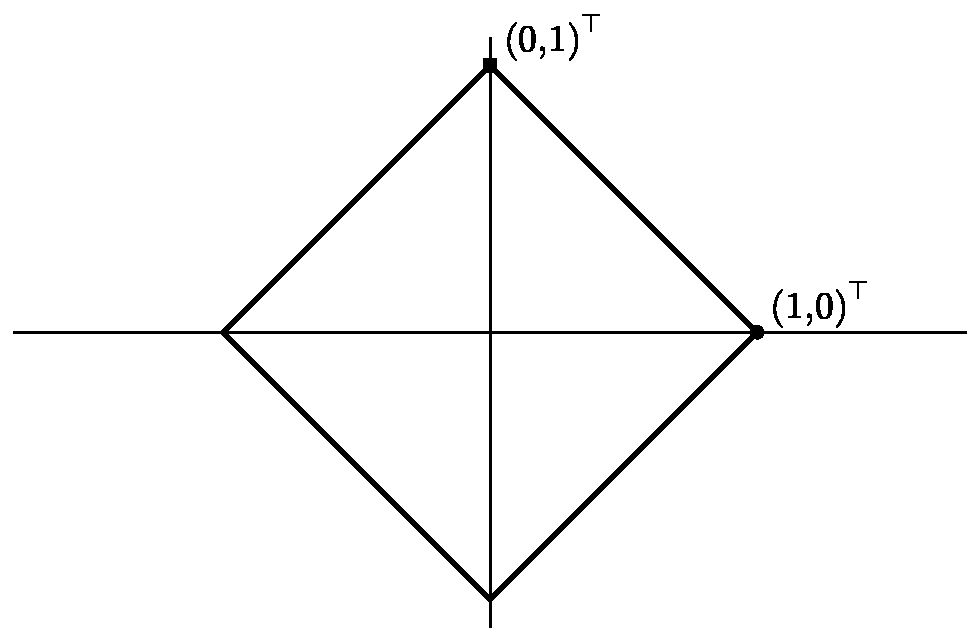
\includegraphics[width=0.25\textwidth]{norm1annotated}&
$\rightarrow$&
\hspace*{-2cm}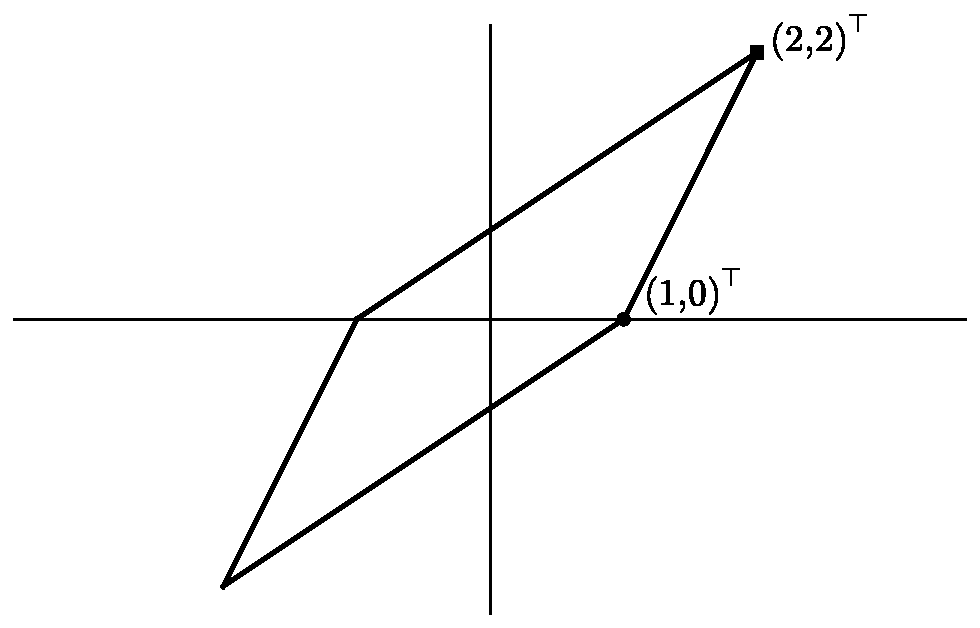
\includegraphics[width=0.25\textwidth]{normA1annotated}&
$\norm{A}_1=4$\\
$2$-norm: &
\hspace*{-1.5cm}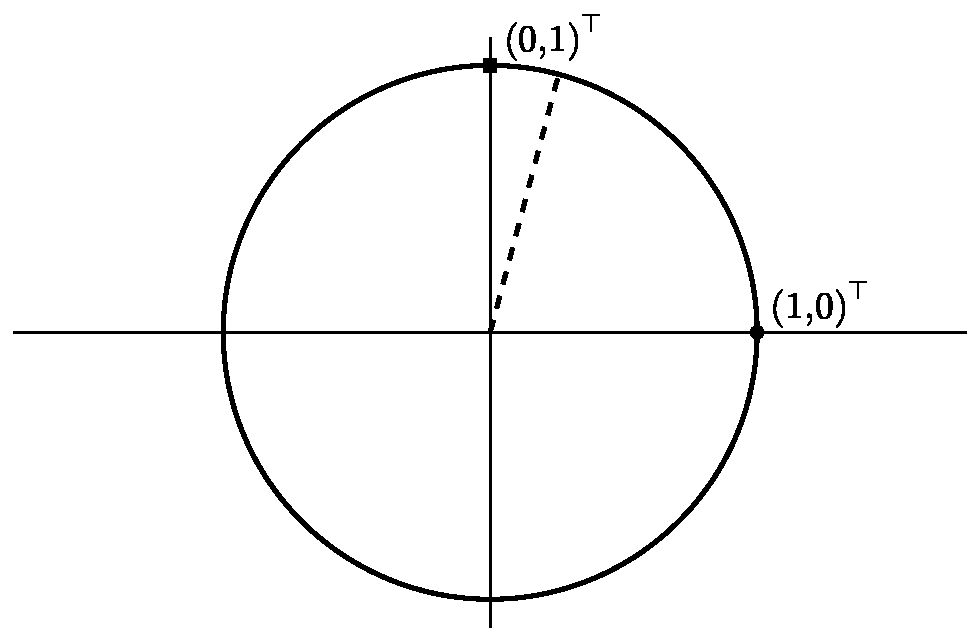
\includegraphics[width=0.25\textwidth]{norm2annotated}&
$\rightarrow$&
\hspace*{-2cm}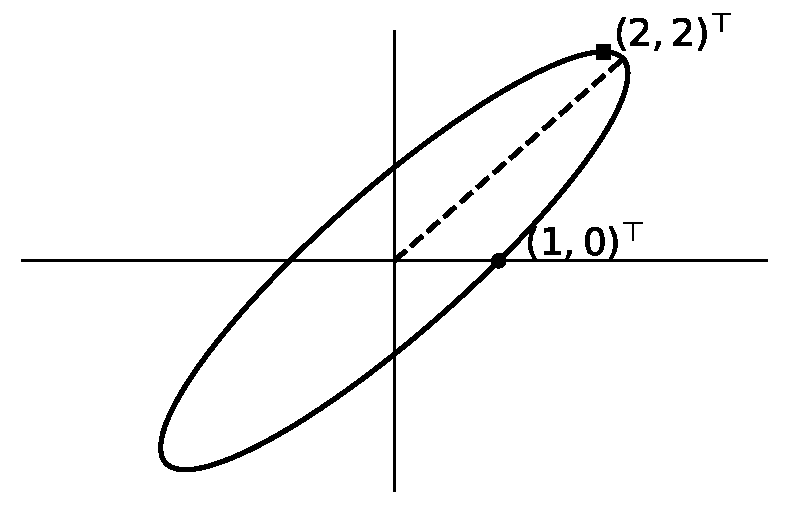
\includegraphics[width=0.25\textwidth]{normA2annotated}&
$\norm{A}_2\approx 2.9208$\\
$\infty$-norm: &
\hspace*{-1.5cm}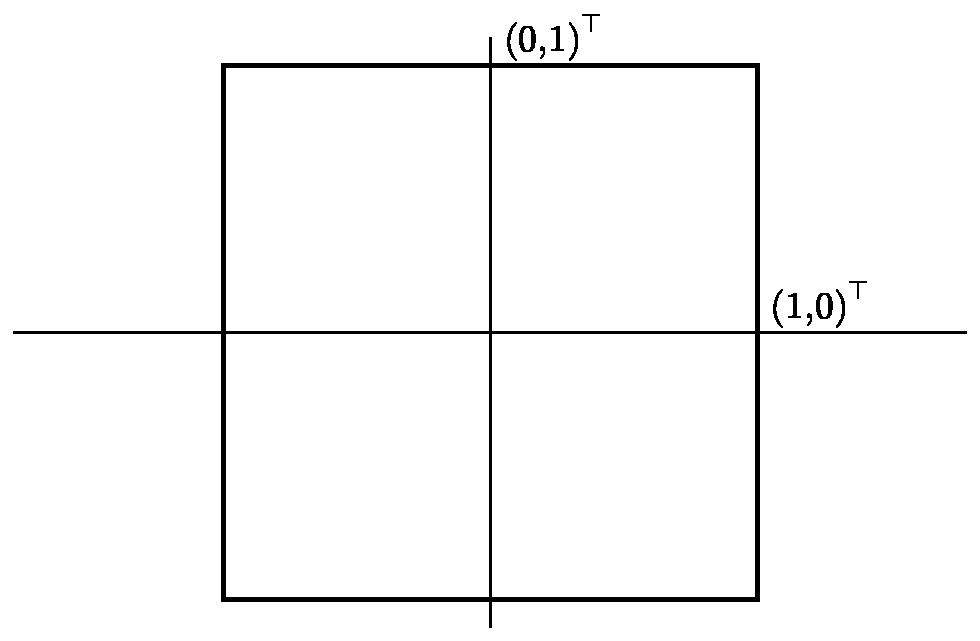
\includegraphics[width=0.25\textwidth]{norminfannotated}&
$\rightarrow$&
\hspace*{-2cm}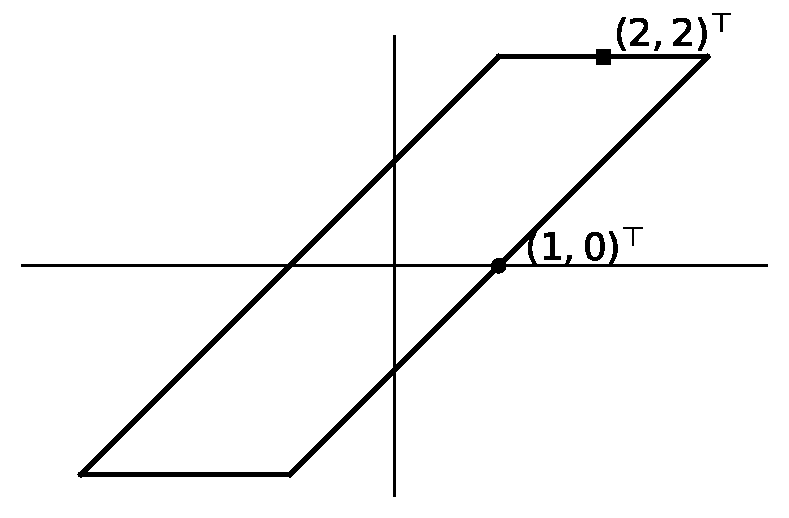
\includegraphics[width=0.25\textwidth]{normAinfannotated}&
$\norm{A}_\infty=3$\\
\end{tabularx}}
\caption{The induced matrix $1$-, $2$-, and $\infty$-norms of $A$.}
\label{figure:InducedNorms}
\end{center}
\end{figure}
\end{example}

\begin{example}\label{example:diagonalpnorm}
The $p$-norm of a diagonal matrix. Let $D$ be the diagonal matrix:
\begin{equation}
D = \begin{bmatrix} d_1\\ &d_2\\&&\ddots\\&&&d_n\end{bmatrix}.
\end{equation}
Then, as in the second row of Figure~\ref{figure:InducedNorms}, the image of the $2$-norm unit sphere under $D$ is an $n$-dimensional ellipse whose semiaxis lengths are given by the numbers $\abs{d_i}$. The unit vectors amplified most by $D$ are those that are mapped to the longest semiaxis of the ellipse, of length $\max_i\{\abs{d_i}\}$. Therefore, we have $\displaystyle \norm{D}_2 = \max_{1\le i\le n}\{\abs{d_i}\}$.

This result for the $2$-norm generalizes to any $p$: if $D$ is diagonal, then $\displaystyle \norm{D}_p = \max_{1\le i\le n}\{\abs{d_i}\}$.
\end{example}

\begin{example}
The $1$-norm of a matrix. If $A$ is any $m\times n$ matrix, then $\norm{A}_1$ is equal to the ``maximum column sum'' of $A$. We explain and derive this result as follows. Write $A$ in terms of its columns:
\begin{equation}
A = \begin{bmatrix} a_1 & \Bigg| & \cdots & \Bigg| & a_n\end{bmatrix},
\end{equation}
where each $a_j$ is an $m$-vector. Consider the diamond-shaped $1$-norm unit ball in $\C^n$, illustrated in Figure~\ref{figure:InducedNorms}. This is the set $\{x\in\C^n:\sum_{j=1}^n\abs{x_j} \le 1\}$. Any vector $Ax$ in the image of this set satisfies:
\begin{equation}
\norm{Ax}_1 = \norm{\sum_{j=1}^nx_ja_j}_1 \le \sum_{j=1}^n\abs{x_j}\norm{a_j}_1 \le \max_{1\le j\le n}\norm{a_j}_1.
\end{equation}
Therefore, the induced matrix $1$-norm satisfies $\norm{A}_1 \le \max_{1\le j\le n}\norm{a_j}_1$. By choosing $x=e_j$, where $j$ maximizes $\norm{a_j}_1$, we attain this bound, and thus the matrix norm is:
\begin{equation}
\norm{A}_1 = \max_{1\le j\le n}\norm{a_j}_1.
\end{equation}
\end{example}

\begin{example}
The $\infty$-norm of a matrix. By much the same argument, it can be shown that the $\infty$-norm of an $m\times n$ matrix is equal to the ``maximum row sum:''
\begin{equation}
\norm{A}_\infty = \max_{1\le i\le m}\norm{a_i^*}_1,
\end{equation}
where $a_i^*$ denotes the $i^{\rm th}$ row of $A$.
\end{example}

Finally, it should be clear that induced norms are submultiplicative, since:
\[
\norm{AB}_p = \sup_{\substack{x\in\C^n\\x\ne0}}\dfrac{\norm{ABx}_p}{\norm{x}_p} = \sup_{\substack{x\in\C^n\\x\ne0\\Bx\ne0}}\dfrac{\norm{ABx}_p}{\norm{Bx}_p}\dfrac{\norm{Bx}_p}{\norm{x}_p} \le \sup_{\substack{y\in\C^n\\y\ne0}}\dfrac{\norm{Ay}_p}{\norm{y}_p}\sup_{\substack{x\in\C^n\\x\ne0}}\dfrac{\norm{Bx}_p}{\norm{x}_p} = \norm{A}_p\norm{B}_p.
\]

\section{Computer Representation of Numbers}

Bits are the smallest piece of information that can be stored in memory on a digital computer. Their role is similar to the role played by atomic particles in quantum physics. The simplest type of numbers we can store with one bit are the Boolean numbers \verb+true+ and \verb+false+. If bits can take on at least two distinct values, such as yes/no or on/off, then Boolean numbers can be represented in one bit.

\subsection{Integers}

The most important integers we can represent on a digital computer are those nearest to $0$. Let $b\in\N$ be a {\em radix}, which is Latin for root or base. Integers can be represented in radix-$b$ as:
\[
\pm(d_kd_{k-1}\cdots d_0)_b = \pm\left(d_kb^k + d_{k-1}b^{k-1} + \cdots + d_0\right),
\]
where the numbers $0\le d_k < b$. In this representation, integers from $0$ to:
\[
(b-1)(b^k+b^{k-1}+\cdots+1) = b^{k+1}-1,
\]
each have a unique signature, and similarly for negative integers from\footnote{We can represent one more negative integer because we only need one $0$.} $-b^{k+1}$ up to $-1$. Using a finite number of bits, a finite number of integers can be represented on a digital computer. As the sign bit behaves just as a Boolean number, we need one extra bit for its inclusion.

\subsection{Fixed-Point Numbers}

Fixed-point numbers are approximations to real numbers $\R$ with a fixed number of digits before the radix point `.' and another fixed number of digits after the radix point:
\[
\pm(d_kd_{k-1}\cdots d_0.d_{-1}\cdots d_{-n})_b = \pm\left(d_kb^k + d_{k-1}b^{k-1} + \cdots + d_0 + d_{-1}b^{-1} + \cdots + d_{-n}b^{-n}\right).
\]
Because fixed-point operations can easily produce results that require more bits than the operands\footnote{If $c = a+b$, then $+$ is the operator and $a$ and $b$ are operands.}, there is possibility for information loss. In scientific computing, fixed-point numbers have fallen from favour because of the need to have scale-invariance in calculations: consider performing any calculation with Planck's constant $h \approx 6.63\times10^{-34}{\rm\,J}\cdot{\rm s}$ and the speed of light squared $c^2 \approx 8.99\times10^{16}{\rm\,m}^2/{\rm s}^2$. This would be an expensive calculation in fixed-point arithmetic, yet it could more easily be done by hand.

\subsection{Floating-Point Numbers}

Modern computers are all binary\footnote{In the 1950's, the Soviets experimented with a balanced ternary (or trinary) computer called Setun, whose bits took the values $\{-1,0,1\}$. The mass production of binary computers has diminished the importance of ternary computing, though it may make a comeback with optical computing.}, whose binary bits can take the value $0$ or $1$. Groups of eight contiguous bits make up a byte; $2^{10}$ bytes make a kilobyte (KB); $2^{20}$ bytes make a megabyte (MB); $2^{30}$ bytes make a gigabyte (GB) and so on and so forth.

The IEEE Standard for Floating-Point Arithmetic (IEEE 754) includes a directive on how to create floating-point numbers to approximate the real numbers on a computer. (Normalized) floating-point numbers are alternative approximations to the reals $\R$ with a fixed number of digits after the radix point {\em multiplied by} a power $p-M$ of the base $2$:
\[
\pm 2^{p-M} \times (1.d_{-1}\cdots d_{-n})_2  = \pm\left(2^{p-M} + d_{-1}2^{p-M-1} + \cdots + d_{-n}2^{p-M-n}\right).
\]
As with the integers and fixed-point numbers, one bit is used to store the sign of the floating-point number, $n$ bits are used for the fractional part known as the {\em mantissa}, and the {\em exponent} $p$ is represented by an unsigned integer. If we use $m$ bits to represent $p$, then we can choose to use the $2^m$ integers in the range $0 \le p < 2^m$. In total, then, we require $1+m+n$ bits to represent the floating-point number. $M$ is known as the {\em exponent bias}.

The IEEE 754 standard prescribes Table~\ref{table:IEEEFloatingPoint} for binary floating-point numbers.

\begin{table}[htdp]
\caption{IEEE 754 standard for binary signed floating-point representation of numbers.}
\begin{center}
\begin{tabular}{ccccccccc}
\hline
Common Name & Base & Digits & Decimal Digits & E Bits & E min & E max & Decimal E max & $M$\\
\hline
Half precision  & $2$ & $10$ & $3.01$ & $5$ & $-14$ & $+15$ & $4.51$ & $15$\\
Single precision  & $2$ & $23$ & $6.92$ & $8$ & $-126$ & $+127$ & $38.23$ & $127$\\
Double precision  & $2$ & $52$ & $15.65$ & $11$ & $-1022$ & $+1023$ & $307.95$ & $1023$\\
\hline
\end{tabular}
\end{center}
\label{table:IEEEFloatingPoint}
\end{table}%

Notice in Table~\ref{table:IEEEFloatingPoint} that the exponent minimum and maximum values fall just short of the maximum allowable range given the number of bits. Subnormal numbers, that is, numbers below $2^{-1022}$ in double precision for example, can only be represented with fewer digits because some of these digits take the surrogate role of extending the power of the exponent.\footnote{Furthermore, subnormal numbers are denormalized and thus start with a $0$ rather than a $1$.} Indeed, the smallest representable number in double precision is $2^{-1022-52} = 2^{-1074}$.

\begin{example}
\begin{itemize}
\item Numbers in double precision, with exponent bias $M=1023$, are stored as:

$\underbrace{\red a}_{\rm 1~sign~bit}\underbrace{\green bbbbbbbbbbb}_{\rm 11~exponent~bits}\underbrace{\blue cccccccccccccccccccccccccccccccccccccccccccccccccccc}_{\rm 52~significand~bits}$

\item For example, $1.0$ is represented by:

{\red0}{\green01111111111}{\blue0000000000000000000000000000000000000000000000000000}

\item and $-29.0$ is:

{\red1}{\green10000000011}{\blue1101000000000000000000000000000000000000000000000000}
\end{itemize}
\end{example}

Floating-point numbers are more versatile than fixed-point numbers because they are distributed in a way which preserves an approximately constant relative precision throughout the range of values they can represent: the density of floating-point numbers accumulates near $0$ and disperses at infinity. In double precision, floating-point numbers are equally distributed in $[\tfrac{1}{2},1)$ with spacing $2^{-53}$, equally distributed in $[1,2)$ with spacing $2^{-52}$, equally distributed in $[2,4)$ with spacing $2^{-51}$ and so on and so forth, and equally distributed in $[\tfrac{1}{4},\tfrac{1}{2})$ with spacing $2^{-54}$, and so on and so forth, as illustrated below.
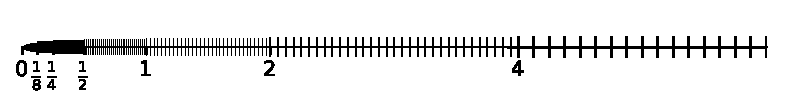
\includegraphics[width=\textwidth]{FloatingPoint}

\subsubsection{How continuous is real life?}

Having decided to approximate real numbers by floating-point numbers on a computer, we might ask how accurately we can represent real life. Avogadro's number $N_A \approx 6.02\times10^{23}{\rm\,molecules}/{\rm mol}$ tells us how many molecules of anything are in one mol. Now, for the sake of the argument, let us take $1{\rm\,m}^3$ of the air with density $\rho = 1.225{\rm\,kg}/{\rm m}^3$ in between you and me. In this cubic meter of air, consisting of roughly $78\%$ nitrogen with a molar mass of $M(N_2) = 28.02{\rm\,g}/{\rm mol}$, we find that there are:
\[
N_A \times M(N_2)^{-1} \times \dfrac{1000{\rm\,g}}{1{\rm\,kg}} \times \rho \times 1{\rm\,m}^3 \approx 2.63\times10^{25}{\rm\,molecules},
\]
of nitrogen in this cubic meter of air. If we assume they are uniformly distributed, then there are only:
\[
\sqrt[3]{2.63\times10^{25}}{\rm\,molecules} \approx 3\times10^8{\rm\,molecules},
\]
lined up in $1{\rm~m}$ in any given direction.

On the other hand, with IEEE double precision floating-point numbers we can distinguish numbers at the scale of one unit of least precision (ulp), that is, the value the least significant digit represents if it is $1$, which is $\approx2.2045\times10^{-16}$ in double precision. Therefore, while we sometimes think of real life as continuous and digital computation as discrete, it is now the case that the level of discreteness on today's computers can be regarded as more refined than real life!

\subsection{The Standard Model}

To store a real number, that is, to obtain a machine representation of a real number, we must truncate the fractional part of the binary expansion of the real number to $n$ bits, the number of bits in the mantissa. This is done by truncating (ignoring all digits after the $n^{\rm th}$ bit) or by rounding. In the latter, if the $(n+1)^{\rm th}$ bit of the expansion of the given number is one, then we round up (taking the first $n$ bits and adding one to the last bit). Otherwise, we simply take the first $n$ bits as in truncation.

Floating-point arithmetic does not obey the usual rules of arithmetic such as the laws of associativity and distributivity. When programming, it is better practice to avoid statements such as:
\begin{verbatim}
if x == .3 then...
\end{verbatim}
Here, rounding errors may mean that the conditional code block is not executed even if the mathematical value of $x$ is $.3$. In this case, it is better to test \verb+if |x-.3| < tol+ where \verb+tol+ is some small tolerance.

For a real number $x$, we denote floating-point approximations to quantities by $\fl(x)$. Using Higham's standard model for floating-point arithmetic~\cite{Higham-02}, we assume that whenever $x$ and $y$ are floating-point numbers and $\circledast$ is one of the four arithmetic operations $+$, $-$, $\times$, or $\div$, we have:
\begin{equation}
\fl(x\circledast y) = (x\circledast y)(1+\delta)^{\pm1},\quad{\rm where}\quad |\delta| \le \epsilon,
\end{equation}
where $\epsilon$ is a unit of least precision.

\begin{lemma}[Higham~\cite{Higham-02}]
If $|\delta_i|\le \epsilon$, and $\rho_i=\pm1$ for $i=1,\ldots,n$, and $n\epsilon<1$, then:
\begin{equation}
\langle n \rangle := \prod_{i=1}^n(1+\delta_i)^{\rho_i} = 1+\theta_n,\qquad |\theta_n| \le \dfrac{n\epsilon}{1-n\epsilon} =:\gamma_n.
\end{equation}
\end{lemma}
\begin{proof}
The proof is by induction.
\end{proof}
The notation $\langle n \rangle$ is useful as a counter to show the accumulation of $n$ relative errors due to rounding. The counters can be manipulated using the rules:
\begin{align}
\langle m\rangle + \langle n\rangle & = \langle\max\{m,n\}\rangle,\\
\langle m\rangle - \langle n\rangle & = \langle\max\{m,n\}\rangle,\\
\langle m\rangle\langle n\rangle & = \langle m+n\rangle,\\
\dfrac{\langle m\rangle}{\langle n\rangle} & = \langle m+n\rangle.
\end{align}

\subsection{Cancellation Error}

Cancellation error is the loss of significant digits when subtracting two nearly equal floating-point numbers. In base-$10$ and with $6$ digits, suppose we wish to find the difference of $1.2345671$ and $1.2345660$. After rounding:
\[
\fl(1.234567-1.234566) = 0.000001 = 1.000000\times10^{-6},
\]
a result which has only one correct digit. This phenomenon can lead to an answer which is completely different from the exact one, especially over the course of a long sequence of operations.

\begin{example}
In base-$10$ and with three digits:
\[
\fl(\fl(\sqrt{9.01})-3.00) = \fl(3.00-3.00) = 0,
\]
which is very different from the exact answer $\approx 1.6662\times10^{-3}$. 

Observe that:
\[
\sqrt{9.01}-3 = (\sqrt{9.01}-3)\dfrac{\sqrt{9.01}+3}{\sqrt{9.01}+3} = \dfrac{0.01}{\sqrt{9.01}+3}.
\]
Calculation of this quantity using the last expression has no cancellation error and leads to $1.67\times10^{-3}$ which is as good as one can expect with three digits.
\end{example}

\begin{example}
Solve $x^2+10^9x-3=0$. By the quadratic formula, the two roots are:
\[
x_- = \dfrac{-10^9-\sqrt{10^{18}+12}}{2},\qquad x_+ = \dfrac{-10^9+\sqrt{10^{18}+12}}{2}.
\]
There is no cancellation in $x_-$ which can be computed accurately in double precision. On the other hand, $x_+$ is a difference of nearly equal numbers. In double precision, the result is exactly zero. As above, a better calculation is:
\[
x_+ = \dfrac{-10^9+\sqrt{10^{18}+12}}{2}\dfrac{10^9+\sqrt{10^{18}+12}}{10^9+\sqrt{10^{18}+12}} = \dfrac{6}{10^9+\sqrt{10^{18}+12}},
\]
which is accurately computed in double precision.
\end{example}

\begin{example}
Consider evaluation of $f(x) = \dfrac{\log(1+x)}{x}$ in a neighbourhood of $x=0$. By l'H\^opital's rule, $f(0)=1$. The na\"ive way to evaluate $f$ suffers from serious cancellation error near $x=0$. In floating-point arithmetic, a better way is the following:
\[
\left\{ \begin{array}{ccc}
\dfrac{\log(\fl(1+x))}{\fl(\fl(1+x)-1)}, & \for & \fl(1+x)\ne 1,\\
1, & \for & \fl(1+x)=1.
\end{array}\right.
\]
Another alternative is to use the (standard) library function $\logop$, defined by its Taylor series near $x=1$ and by $\log\fl(1+x)$ sufficiently far away to cause no loss of accuracy, such that $f(x) = \logop(x)/x$. Figure~\ref{figure:log1pdx} shows the relative error in approximating $f$ using all three methods.
\begin{figure}[htbp]
\begin{center}
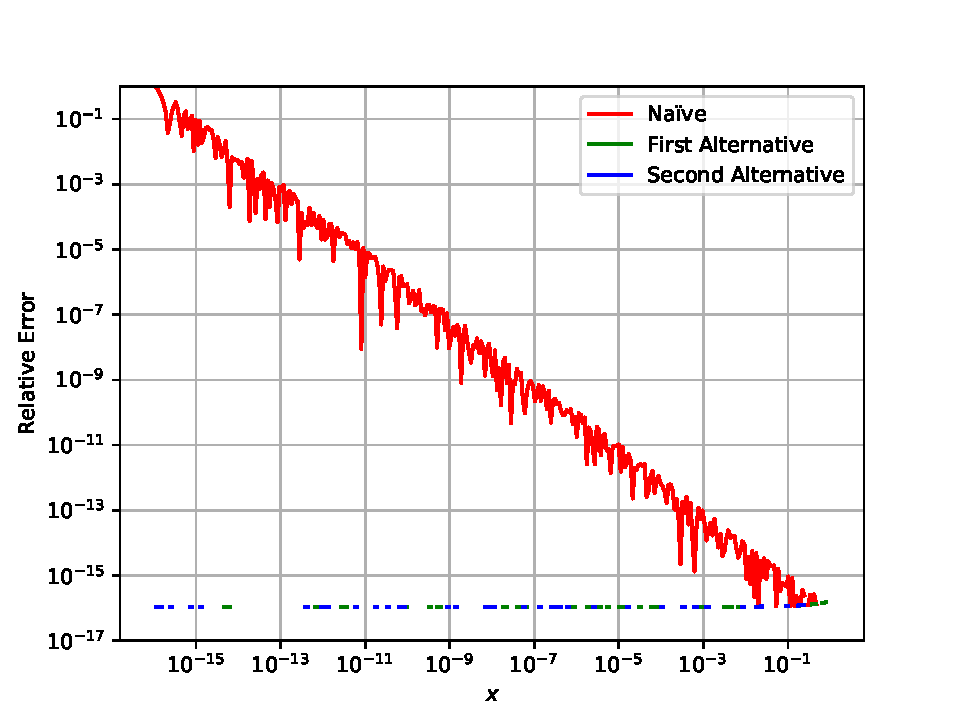
\includegraphics[width=0.65\textwidth]{log1pdx}
\caption{Comparison of the na\"ive and alternative methods for computing $f(x) = \frac{\log(1+x)}{x}$.}
\label{figure:log1pdx}
\end{center}
\end{figure}
\end{example}

Sums of floating-point numbers are ubiquitous in scientific computing. They occur when evaluating inner products, norms, means, variances, and all kinds of nonlinear functions. Although at first sight summation might appear to offer little scope for algorithmic ingenuity, the usual ``recursive summation'' (with various orderings) is just one of a variety of possible techniques. We describe several summation methods and their error analyses in the next example. No one method is uniformly more accurate than the others, but some guidelines can be given on the choice of method in particular cases.

\begin{example}
Consider the computation of $\displaystyle S_n = \sum_{i=1}^nx_i$ using the following algorithms:
\begin{enumerate}
\item Recursive summation, where we set $s=0$ and recursively add $x_i$ to $s$ for $i=1,\ldots,n$; and,
\item Pairwise summation (also know as cascade summation), where the $x_i$ are summed in pairs according to:
\[
y_i = x_{2i-1}+x_{2i},\quad{\rm for}\quad i=1,\ldots\lfloor\tfrac{n}{2}\rfloor,\quad (y_{(n+1)/2} = x_n\hbox{ if }n\hbox{ is odd}),
\]
and this pairwise summation repeats recursively on the $y_i$, obtaining the sum in $\lceil\log_2n\rceil$ stages.
\end{enumerate}
Using the standard model, recursive summation leads to the accumulation of $\langle n-1\rangle$ rounding errors, while pairwise summation only leads to the accumulation of $\langle \lceil\log_2 n\rceil\rangle$ rounding errors. For example, for recursive summation of $S_8$, we have:
\begin{align*}
\fl(S_8) & = \fl(\fl(\fl(\fl(\fl(\fl(\fl(x_1+x_2)+x_3)+x_4)+x_5)+x_6)+x_7)+x_8),\\
& = (((((((x_1+x_2)\langle1\rangle+x_3)\langle1\rangle+x_4)\langle1\rangle+x_5)\langle1\rangle+x_6)\langle1\rangle+x_7)\langle1\rangle+x_8)\langle1\rangle,\\
& = (((((((x_1+x_2)\langle2\rangle+x_3\langle1\rangle)+x_4)\langle1\rangle+x_5)\langle1\rangle+x_6)\langle1\rangle+x_7)\langle1\rangle+x_8)\langle1\rangle,\\
& = ((((((x_1+x_2+x_3)\langle2\rangle+x_4)\langle1\rangle+x_5)\langle1\rangle+x_6)\langle1\rangle+x_7)\langle1\rangle+x_8)\langle1\rangle,\\
& = (((((x_1+x_2+x_3+x_4)\langle3\rangle+x_5)\langle1\rangle+x_6)\langle1\rangle+x_7)\langle1\rangle+x_8)\langle1\rangle,\\
& = ((((x_1+x_2+x_3+x_4+x_5)\langle4\rangle+x_6)\langle1\rangle+x_7)\langle1\rangle+x_8)\langle1\rangle,\\
& = (((x_1+x_2+x_3+x_4+x_5+x_6)\langle5\rangle+x_7)\langle1\rangle+x_8)\langle1\rangle,\\
& = ((x_1+x_2+x_3+x_4+x_5+x_6+x_7)\langle6\rangle+x_8)\langle1\rangle,\\
& = S_8\langle7\rangle.
\end{align*}
On the other hand, for pairwise summation of $S_8$, we have:
\begin{align*}
\fl(S_8) & = \fl(\fl(\fl(x_1+x_2) + \fl(x_3+x_4)) + \fl(\fl(x_5+x_6) + \fl(x_7+x_8))),\\
& = (((x_1+x_2)\langle1\rangle + (x_3+x_4)\langle1\rangle)\langle1\rangle + ((x_5+x_6)\langle1\rangle + (x_7+x_8)\langle1\rangle)\langle1\rangle)\langle1\rangle,\\
& = ((x_1+x_2+x_3+x_4)\langle2\rangle + (x_5+x_6+x_7+x_8)\langle2\rangle)\langle1\rangle,\\
& = S_8\langle3\rangle.
\end{align*}
Note that there are even other alternative methods, and even changing the direction of the recursive summation can lead to an improvement in certain sums. For example, if the sequence $\abs{x_i}$ is decreasing, the reverse recursive summation can be even more accurate than pairwise summation, exhibiting no error growth with $n$! This shows that when we start making assumptions on $x_i$, the error analysis with counters can be made more precise. This also shows that no algorithm is uniformly more accurate. Figure~\ref{figure:summation} compares forward/reverse recursive and pairwise summation for a given sequence.
\begin{figure}[htbp]
\begin{center}
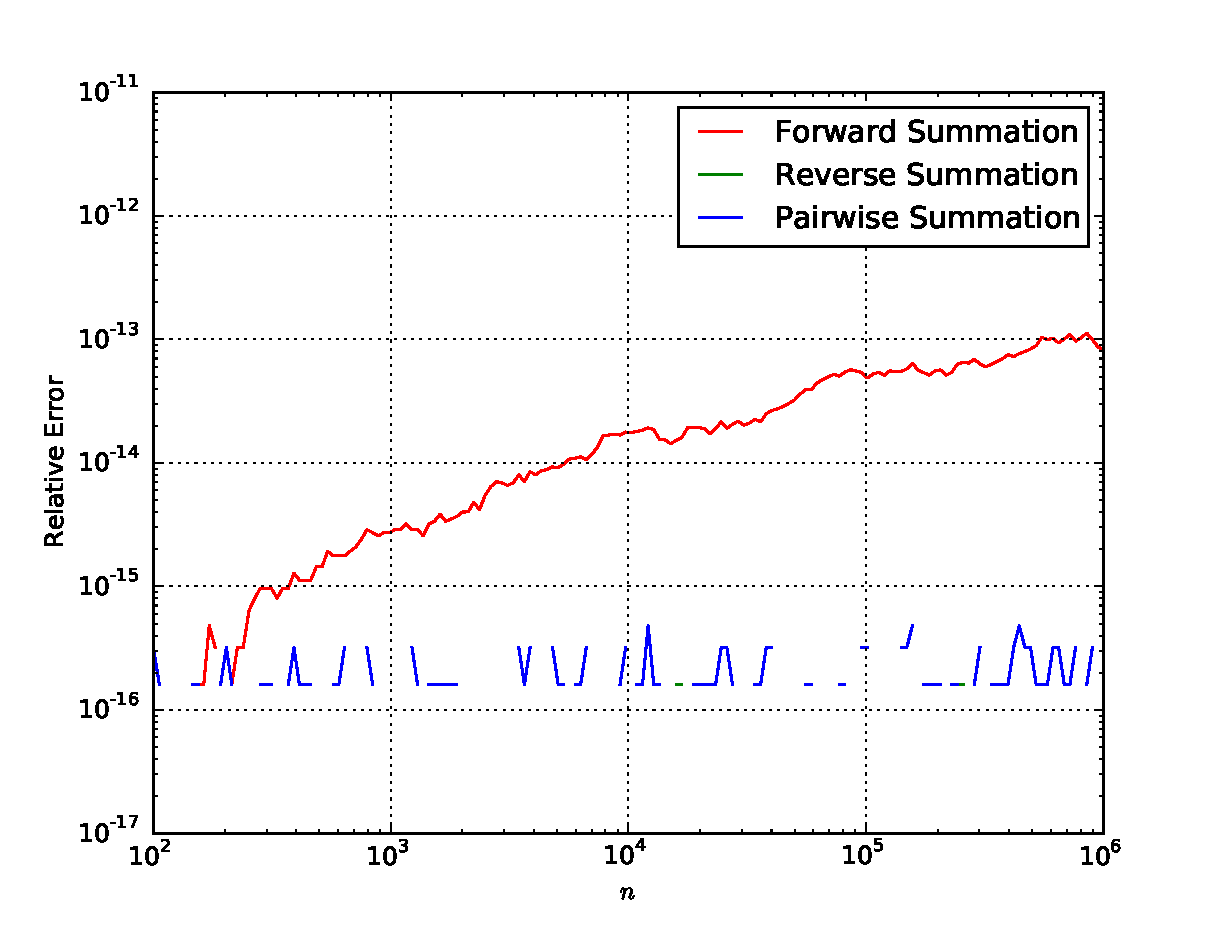
\includegraphics[width=0.65\textwidth]{summation}
\caption{Comparison of the recursive and pairwise summation algorithms for $\displaystyle S_n = \sum_{i=1}^n\dfrac{(-1)^i}{i}$.}
\label{figure:summation}
\end{center}
\end{figure}
\end{example}

\section{Conditioning and Stability}

A problem typically has an input and an output. The input consists of a set of data, say, the coefficients of some equation, and the output of another set of numbers uniquely determined by the input, say, all the roots of the equation in some prescribed order. If we collect the input in a vector $x\in X$, and the output in the vector $y\in Y$, where $X$ and $Y$ are normed vector spaces, we may thus think of a problem as a map $f$, given by:
\begin{equation}
f:X\to Y,\quad y = f(x).
\end{equation}
What we are interested in is the sensitivity of the map $f$ at some given point $x$ to a small perturbation of $x$, that is, how much bigger (or smaller) is the perturbation in $y$ compared to the perturbation in $x$? In particular, we wish to measure the degree of sensitivity by a single number -- the {\em condition number} of the map $f$ at the point $x$. We emphasize that, as we perturb $x$, the function $f$ is always assumed to be evaluated exactly, with infinite precision. The condition of $f$, therefore is an inherent property of the map $f$ and does not depend on any algorithmic considerations concerning its implementation in finite precision on a computer.

This is not to say that knowledge of the condition of a problem is irrelevant to any algorithmic solution of the problem. On the contrary, the reason is that quite often the {\em computed solution} $y^*$, using a specific algorithm in finite precision, can be demonstrated to be the {\em exact} solution to a ``nearby'' problem, that is:
\begin{equation}
y^* = f(x^*),
\end{equation}
where $x^*$ is a point close to the given data $x$:
\begin{equation}
x^* = x+\Delta x,
\end{equation}
and moreover, the distance $\norm{\Delta x}_X$ of $x^*$ to $x$ can be estimated in terms of the machine precision. Therefore, if we know how strongly (or weakly) the map $f$ reacts to a small perturbation, such as $\Delta x$, we can say something about the error $\norm{y^*-y}_Y$ in the solution caused by this perturbation. This, indeed, is an important technique of error analysis -- know as {\em backward error analysis} -- which was pioneered in the 1950's by Givens, Lanczos, and Wilkinson.

\begin{example}
\begin{enumerate}
\item For a given matrix $A\in\R^{m\times n}$, define the problem of matrix-vector multiplication $f:\R^n\to\R^m$ with the Euclidean norms on the input and output:
\begin{equation}
f(x) = Ax.
\end{equation}
This problem encodes the sensitivity of matrix-vector multiplication to perturbations in the {\em vector}.
\item For a given vector $x\in\R^n$, define the problem of matrix-vector multiplication $f:\R^{m\times n}\to\R^m$ with the (induced) $2$-norms on the input and output:
\begin{equation}
f(A) = Ax.
\end{equation}
This problem encodes the sensitivity of matrix-vector multiplication to perturbations in the {\em matrix}.
\item Define the whole problem of matrix-vector multiplication $f:\R^{m\times n}\times\R^n\to\R^m$:
\begin{equation}
f(A,x) = Ax.
\end{equation}
Clearly, we can attach the $2$-norm to the output. For the input, we attach the norm:
\begin{equation}
\norm{(A,x)} = \max\{\norm{A}_2,\norm{x}_2\}.
\end{equation}
This problem encodes the sensitivity of matrix-vector multiplication to perturbations in {\em both} the matrix and the vector.
\item For a given vector $x\in\R^n$, define the problem of inverse matrix-vector multiplication (solving a linear system) $f:\R^n\to\R^m$ with the (induced) $2$-norms on the input and output:
\begin{equation}
f(x) = A^{-1}x.
\end{equation}
This problem encodes the sensitivity of matrix inversion to perturbations in the {\em vector}.
\end{enumerate}
\end{example}

Maps $f$ between more general spaces (in particular, function spaces) have also been considered from the point of view of conditioning, but eventually, these spaces are reduced to finite-dimensional spaces for practical implementation.

We can measure the error using either {\em absolute} or {\em relative} error. The absolute error for the input $x$ perturbed by $\Delta x$ is:
\begin{equation}
\Delta y = f(x+\Delta x) - f(x),
\end{equation}
while the relative error (if $f:X\to\R$ has one-dimensional output) is:
\begin{equation}
\dfrac{\Delta y}{y} = \dfrac{f(x+\Delta x)-f(x)}{f(x)},\qquad y\ne 0.
\end{equation}

\begin{definition}
The {\em absolute condition number} of a problem is a measure of how much the absolute error in the input is magnified to cause absolute error in the output:
\begin{equation}
\cond_{\rm abs}(f,\epsilon) := \sup_{\norm{\Delta x}_X \le \epsilon}\dfrac{\norm{f(x+\Delta x)-f(x)}_Y}{\norm{\Delta x}_X}.
\end{equation}
\end{definition}
We see that by this definition, the condition number gives us a bound on the absolute error subject to an $\epsilon$-perturbation in the input:
\begin{equation}
\norm{f(x+\Delta x)-f(x)}_Y \le \cond_{\rm abs}(f,\epsilon)\norm{\Delta x}_X.
\end{equation}

\begin{definition}
The {\em relative condition number} of a problem is a measure of how much the relative error in the input is magnified to cause relative error in the output:
\begin{equation}
\cond_{\rm rel}(f,\epsilon) := \sup_{\norm{\Delta x}_X \le \epsilon}\dfrac{\norm{f(x+\Delta x)-f(x)}_Y}{\norm{\Delta x}_X}\dfrac{\norm{x}_X}{\norm{f(x)}_Y}.
\end{equation}
\end{definition}
We see that by this definition, the condition number gives us a bound on the relative error subject to an $\epsilon$-perturbation in the input:
\begin{equation}
\dfrac{\norm{f(x+\Delta x)-f(x)}_Y}{\norm{f(x)}_Y} \le \cond_{\rm rel}(f,\epsilon)\dfrac{\norm{\Delta x}_X}{\norm{x}_X}.
\end{equation}

\begin{example}
Consider the problem of evaluating the function $f\in C^1(D)$ at some point $x\in D\subset\R$. The relative condition number is:
\[
\cond_{\rm rel}(f,\epsilon) = \sup_{\abs{\Delta x} \le \epsilon}\dfrac{\abs{f(x+\Delta x)-f(x)}}{\abs{\Delta x}}\dfrac{\abs{x}}{\abs{f(x)}}.
\]
If the perturbations are truly small, then the limiting value as $\epsilon\to0$ can be taken as a sensible approximation of the relative condition number:
\[
\cond_{\rm rel}(f,\epsilon) \approx \lim_{\epsilon\to0} \cond_{\rm rel}(f,\epsilon) = \abs{\dfrac{xf'(x)}{f(x)}}.
\]
\end{example}

\begin{definition}
The $p$-norm {\em condition number of a square matrix} is defined by:
\begin{equation}
\cond_p(A) := \norm{A}_p\norm{A^{-1}}_p.
\end{equation}
\end{definition}

The condition number of a matrix gives a least upper bound on the relative condition number of the problems of matrix-vector multiplication and solution of linear systems described earlier.

\begin{example}
\begin{enumerate}
\item For the problem of matrix-vector multiplication subject to perturbations in the vector, the relative condition number is:
\[
\cond_{\rm rel}(f,\epsilon) = \sup_{\norm{\Delta x}_p \le \epsilon}\dfrac{\norm{A(x+\Delta x)-Ax}_p}{\norm{\Delta x}_p}\dfrac{\norm{x}_p}{\norm{Ax}_p} = \dfrac{\norm{x}_p}{\norm{Ax}_p}\sup_{\norm{\Delta x}_p \le \epsilon}\dfrac{\norm{A\Delta x}_p}{\norm{\Delta x}_p} = \dfrac{\norm{x}_p}{\norm{Ax}_p}\norm{A}_p.
\]
The condition number is bounded by $\cond_p(A)$ since:
\[
\cond_{\rm rel}(f,\epsilon) = \dfrac{\norm{A^{-1} Ax}_p}{\norm{Ax}_p}\norm{A}_p \le \dfrac{\norm{A^{-1}}_p\norm{Ax}_p}{\norm{Ax}_p}\norm{A}_p = \cond_p(A).
\]
\item For the problem of solution of linear systems subject to perturbations in the vector, the relative condition number is:
\begin{align*}
\cond_{\rm rel}(f,\epsilon) & = \sup_{\norm{\Delta x}_p \le \epsilon}\dfrac{\norm{A^{-1}(x+\Delta x)-A^{-1}x}_p}{\norm{\Delta x}_p}\dfrac{\norm{x}_p}{\norm{A^{-1}x}_p},\\
& = \dfrac{\norm{x}_p}{\norm{A^{-1}x}_p}\sup_{\norm{\Delta x}_p \le \epsilon}\dfrac{\norm{A^{-1}\Delta x}_p}{\norm{\Delta x}_p} = \dfrac{\norm{x}_p}{\norm{A^{-1}x}_p}\norm{A^{-1}}_p.
\end{align*}
The condition number is {\em still} bounded by $\cond_p(A)$ since:
\[
\cond_{\rm rel}(f,\epsilon) = \dfrac{\norm{AA^{-1}x}_p}{\norm{A^{-1}x}_p}\norm{A^{-1}}_p \le \dfrac{\norm{A}_p\norm{A^{-1}x}_p}{\norm{A^{-1}x}_p}\norm{A^{-1}}_p = \cond_p(A).
\]
\end{enumerate}
\end{example}

\begin{example}
The Hilbert matrix is the square matrix of dimension $n$ with entries $[H_n]_{i,j} = \dfrac{1}{i+j-1}$. This symmetric matrix has an extremely large $2$-norm condition number. A result due to Szeg\H o states that:
\begin{equation}\label{eq:Szego}
\cond_2(H_n) \sim \dfrac{\pr(\sqrt{2}+1)^{4n+4}}{2^{\frac{15}{4}}\sqrt{\pi n}},\quad{\rm as}\quad n\to\infty.
\end{equation}
Table~\ref{table:Hilbert} shows some numerical values of the condition number of $H_n$ with respect to the dimension $n$. In fact, the rapid growth of the condition number implies that beyond $n=12$, neither the matrix-vector product nor the solution of a linear system can be computed with any reliability in $64$-bit floating-point arithmetic.
\begin{table}[htdp]
\caption{The $2$-norm condition number of Hilbert matrices.}
\begin{center}
\begin{tabular}{rl@{$\times$}ll@{$\times$}l}
\hline
$n$ & \multicolumn{2}{c}{$\cond_2(H_n)$} & \multicolumn{2}{c}{Estimate~\eqref{eq:Szego}}\\
\hline
$5$ & $4.76607250242561$ & $10^5$ & $2.88200032765989$ & $10^{7}$\\
$10$ & $1.6026286870216889$ & $10^{13}$ & $9.219189347346499$ & $10^{14}$\\
$15$ & $6.116565791619838$ & $10^{20}$ & $3.405342605196914$ & $10^{22}$\\
$20$ & $2.4521565858153033$ & $10^{28}$ & $1.334151505013483$ & $10^{30}$\\
$25$ & $1.0096548421909462$ & $10^{36}$ & $5.398384956972705$ & $10^{37}$\\
$30$ & $4.227806388187525$ & $10^{43}$ & $2.2293945465873128$ & $10^{45}$\\
$35$ & $1.7910802642986633$ & $10^{51}$ & $9.337427577656723$ & $10^{52}$\\
$40$ & $7.652913898310316$ & $10^{58}$ & $3.951345265521789$ & $10^{60}$\\
\hline
\end{tabular}
\end{center}
\label{table:Hilbert}
\end{table}%
\end{example}

Note that this example illustrates an {\em extreme} scenario, where the condition number of the family of Hilbert matrices grows extremely rapidly with respect to the dimension $n$. Such problems are deemed {\em ill-conditioned}. In many cases of interest, the condition number will be low enough for us to obtain reasonable accuracy in floating-point arithmetic. These problems are deemed {\em well-conditioned}.

\begin{remark}\label{remark:ConditionNumberFactorization}
The condition number of the {\em problem} is different from the condition number of the {\em algorithm} we use to solve the problem. For example, suppose we wish to solve the linear system:
\[
Ax = b.
\]
One useful approach is to develop a factorization of $A = BC$, where the inverses of the matrices $B$ and $C$ can be applied to the vector $b$ in fewer operations than a dense solve. In this case, the algorithm consists of:
\begin{enumerate}
\item Solve for $y := B^{-1}b$; and,
\item Solve for $x = C^{-1}y$.
\end{enumerate}
Using matrix inequalities, we can compare condition numbers of the problem and the algorithm:
\begin{align*}
\cond_p(A) = \cond_p(BC) & = \norm{BC}_p\norm{(BC)^{-1}}_p = \norm{BC}_p\norm{C^{-1}B^{-1}}_p,\\
& \le \norm{B}_p\norm{C}_p\norm{C^{-1}}_p\norm{B^{-1}}_p = \cond_p(B)\cond_p(C).
\end{align*}
Therefore, the condition number of the algorithm, consisting of the product $\cond_p(B)\cond_p(C)$, is {\em at least as large} as the condition number of the problem, but depending on our choice of the factorization $BC$, it could be much worse!
\end{remark}

Algorithms that do not needlessly generate ill-conditioning, that is, algorithms for which the condition number of the problem and the condition number of algorithm do not differ egregiously, are said to be stable algorithms. While this concept is rather vague, in certain instances the stability of a given algorithm can be made precise.

\section{Theorems of Calculus}

\begin{theorem}[Mean Value Theorem]
If $f\in C([a,b])$, where $a<b$, and if $f\in C^1(a,b)$, then $\exists c\in(a,b)$ for which:
\[
f'(c) = \dfrac{f(b)-f(a)}{b-a}.
\]
\end{theorem}

\begin{theorem}[Integral Mean Value Theorem]
If $f,g\in C([a,b])$, and $g(x)\ge0$ on this interval, then $\exists c\in(a,b)$ for which:
\[
\int_a^bf(x)g(x)\ud x = f(c)\int_a^bg(x)\ud x.
\]
\end{theorem}

\begin{theorem}[Intermediate Value Theorem]
If $f\in C([a,b])$ and $c$ is any number between $f(a)$ and $f(b)$ then there is at least one number $\xi\in(a,b)$ such that $f(\xi) = c$.
\end{theorem}

\begin{theorem}[Taylor's Theorem]\label{eq:Taylor}
Let $k\in\N$ and let the function $f$ be $k$ times differentiable at the point $a$. Then Taylor's approximation is:
\[
f(x) = f(a) + f'(a)(x-a) + \cdots + \dfrac{f^{(k)}(a)}{k!}(x-a)^k + r_k(x),
\]
where $r_k(x)$ is a remainder term. The formul\ae~for $r_k(x)$ are due to several others:
\begin{description}
\item[Peano form of the remainder] $r_k(x) = o(|x-a|^k)$, that is, as $x\to a$, the remainder tends to zero faster than the $k^{\rm th}$ power of the difference;
\item[Lagrange form of the remainder] if $f\in C^{k+1}(a,x)$ and if $f\in C^k([a,x])$, then $\exists c\in(a,x)$ for which:
\[
r_k(x) = \dfrac{f^{(k+1)}(c)}{(k+1)!}(x-a)^{k+1};\hbox{ and},
\]
\item[Cauchy form of the remainder] if $f\in C^{k+1}(a,x)$ and if $f\in C^k([a,x])$, then $\exists c\in(a,x)$ for which:
\[
r_k(x) = \dfrac{f^{(k+1)}(c)}{k!}(x-c)^{k}(x-a).
\]
\end{description}
\end{theorem}
Each form of the remainder in Taylor's theorem is useful in a different context.

\section{Asymptotic Analysis and Complexity}

It is important to be able to describe the characteristics of numerical algorithms. While wall time of an algorithm is certainly important, mathematically it is interesting to understand how the algorithm scales with increasing, say, the problem dimension $n$. If it doubles, 
\begin{itemize}
\item how much longer can we expect to wait?
\item how much larger do the errors grow?
\item how much more space must be allocated to carry out the extra computations?
\end{itemize}

To this end, we will find that notation from asymptotic analysis will be useful. This is an extension of our natural capabilities of estimation, and is even more effective when coupled with the $p$-norms.

\begin{definition}
\begin{enumerate}
\item If there exists an $0<M<\infty$ such that:
\begin{equation}
|f(z)| \le M|g(z)|,\quad{\rm as}\quad z\to z_0,~z\in D,
\end{equation}
then we say $f(z) = \OO(g(z))$ ($f$ is on the order of $g$) as $z\to z_0$. Equivalently:
\begin{equation}
\lim_{\substack{z\to z_0\\z\in D}}\abs{\dfrac{f(z)}{g(z)}} = M.
\end{equation}
\item If for all $0<M<\infty$:
\begin{equation}
|f(z)| < M|g(z)|,\quad{\rm as}\quad z\to z_0,~z\in D,
\end{equation}
then we say $f(z) = o(g(z))$ as $z\to z_0$. Equivalently:
\begin{equation}
\lim_{\substack{z\to z_0\\z\in D}}\abs{\dfrac{f(z)}{g(z)}} = 0.
\end{equation}
\item If $f(z) = \OO(g(z))$ with the constant $M=1$, then we say $f(z) \sim g(z)$ ($f$ is asymptotic to $g$) as $z\to z_0$. Equivalently:
\begin{equation}
\lim_{\substack{z\to z_0\\z\in D}}\abs{\dfrac{f(z)}{g(z)}} = 1.
\end{equation}
\end{enumerate}
\end{definition}

\begin{example}
Using Taylor's theorem and the geometric series, we know that:
\begin{enumerate}
\item $\sin x \sim x,\quad{\rm as}\quad x\to0$;
\item $\cos x = 1 + \OO(x^2),\quad{\rm as}\quad x\to0$;
\item $\dfrac{e^x-1}{x} \sim 1,\quad{\rm as}\quad x\to0$; and,
\item $\displaystyle \dfrac{1}{1-x^2} = -\dfrac{1}{x^2(1-1/x^2)} = -\dfrac{1}{x^2}\sum_{n=0}^\infty\left(\dfrac{1}{x^2}\right)^n = -\dfrac{1}{x^2}+o(x^{-3})\quad{\rm as}\quad x\to\infty$.
\end{enumerate}
\end{example}

\section{Simple Numerical Algorithms}

\subsection{Horner's Rule}

Horner's rule~\cite{Horner-109-308-19} is an algorithm for evaluating polynomials in the monomial basis. Let $p_n(x) = \sum_{k=0}^n c_kx^k$.
\begin{algorithm}[Horner~\cite{Horner-109-308-19}]~
\begin{description}
\item[Step 1:] Initialization:

{\tt S = c[n]}.
\item[Step 2:] The main loop:
\begin{verbatim}
for k = n-1:-1:0
    S = c[k] + x*S
end
\end{verbatim}
\end{description}
$S$ is the result of evaluating $p_n$ at the point $x$.
\end{algorithm}
This algorithm is derived by re-expressing the polynomial $p_n$ as:
\[
p_n(x) = c_0 + x(c_1 + x(c_2 + \cdots + x(c_{n-1}+c_nx))).
\]
Horner's rule requires:
\begin{itemize}
\item $n$ additions and $n$ multiplications, or $\OO(n)$ flops; and,
\item $1$ unit of storage during execution, or $\OO(1)$ storage.
\end{itemize}
It is an example of a perfectly fine algorithm for numerically evaluating polynomials in the monomial basis.

\subsection{Bisection Method}

The bisection method is used to compute a solution of the equation $f(x) = 0$ in an interval $x\in[a,b]$. Based on the Intermediate Value Theorem, a continuous function $f$ which changes sign on $[a,b]$ has at least one zero in the open interval $(a,b)$. Bisection adds to this a comparison with the function evaluated at the midpoint $c = \frac{a+b}{2}$ to determine in which interval to continue to subdivide. Pseudo-code for the algorithm is as follows:

\begin{algorithm}[Bisection]~\\
\begin{description}
\item[Step 1:] Initialization:
\begin{verbatim}
fa = f(a)
fb = f(b)
if fa*fb > 0
    error("Bisection cannot guarantee a root")
end
if fa == 0
    return a
elseif fb == 0
    return b
end
absbma = abs(b-a)
\end{verbatim}
\item[Step 2:] The main loop:
\begin{verbatim}
while abs(b-a) > absbma*tol
    c = (a+b)/2
    fc = f(c)
    if fa*fc > 0 # f(a) and f(c) have the same sign
        a = c
        fa = fc
    elseif fa*fc < 0 # f(a) = f(c) have opposite sign
        b = c
        fb = fc
    else # fa*fc == 0 which means f(c) == 0.
    	return c
    end
end
c = (a+b)/2
return c
\end{verbatim}
\end{description}
$c$ is the result of bisecting until we find a zero.
\end{algorithm}

If we let $c_n$ denote the coordinate of the $n^{\rm th}$ iteration of the bisection method and $\displaystyle x^* = \lim_{n\to\infty} c_n$, then it is straightforward to reason that:
\begin{equation}\label{eq:bisectionerror}
\abs{x^* - c_n} \le \frac{\abs{b-a}}{2^n},
\end{equation}
since the error is at least halved after every iteration.

\section{Problems}

\begin{enumerate}

\item Vector and matrix $p$-norms are related by various inequalities, often involving the dimensions $m$ or $n$. For each of the following, verify the inequality and give an example of a nonzero vector or matrix (for general $m$, $n$) for which equality is achieved. In this problem, $x$ is an $n$-vector and $A$ is an $m\times n$ matrix.
\begin{enumerate}
\item $\norm{x}_\infty \le \norm{x}_2$;
\item $\norm{x}_2 \le \sqrt{n}\norm{x}_\infty$;
\item $\norm{A}_\infty \le \sqrt{n}\norm{A}_2$; and,
\item $\norm{A}_2 \le \sqrt{m}\norm{A}_\infty$.
\end{enumerate}

\item Let the matrix $A = uv^\top$ be the {\em outer product} of the vectors $u\in\R^m$ and $v\in\R^n$ such that $A_{i,j} = u_iv_j$. Use the Cauchy--Schwarz inequality to show that $\norm{A}_2 = \norm{u}_2\norm{v}_2$.

\item Convert:
\begin{itemize}
\item the binary number $(0.111101)_2$ into decimal; and,
\item the octal number $(0.3416)_8$ into binary.
\end{itemize}

\item \begin{enumerate}
\item Write a {\sc Julia} function {\tt bisection(a,b,f,tol)} that implements the bisection method;
\item Use Eq.~\eqref{eq:bisectionerror} to determine precisely the number $n$ of iterations that are required to reduce the error $\abs{x^*-c_n}$ below a tolerance $\varepsilon>0$;
\item Write a new function, say {\tt bisection2(a,b,f,tol)}, that implements the bisection method with a {\tt for} loop using precisely $n$ iterations (no fewer, no more) rather than the {\tt while} loop; and,

\item Use both functions with a tolerance {\tt tol = eps()} to compute a zero of:
\begin{itemize}
\item $f(x) = 2\cos(2x)+x^3-e^x$ in $[0,5]$; and,
\item $g(x) = \sin(15x)$ in $[-1,1]$.
\end{itemize}
Report and explain your results.
\end{enumerate}

\item The condition number of the Hilbert matrices grows so rapidly that using a built-in computer function \verb+cond+ will {\em not} accurately compute the condition number past about $n=12$. Instead, use the definition of $\cond_2(A) := \norm{A}_2\norm{A^{-1}}_2$ together with the inverse Hilbert matrices with elements given by:
\[
[H_n^{-1}]_{i,j} = (-)^{i+j}(i+j-1)\binom{n+i-1}{n-j}\binom{n+j-1}{n-i}\binom{i+j-2}{i-1}^2,
\]
following these steps.
\begin{enumerate}
\item Use properties of binomial coefficients to simplify the expression to the following:
\[
[H_n^{-1}]_{i,j} = \dfrac{(-)^{i+j}n^2}{i+j-1}\binom{n-1}{i-1}\binom{n-1}{j-1}\binom{n+i-1}{i-1}\binom{n+j-1}{j-1};
\]
\item Derive the recurrences:
\[
[H_n^{-1}]_{i,j} = -\dfrac{i+j-2}{i+j-1}\cdot\dfrac{n-i+1}{i-1}\cdot\dfrac{n+i-1}{i-1}\cdot[H_n^{-1}]_{i-1,j},
\]
and:
\[
[H_n^{-1}]_{i,j} = -\dfrac{i+j-2}{i+j-1}\cdot\dfrac{n-j+1}{j-1}\cdot\dfrac{n+j-1}{j-1}\cdot[H_n^{-1}]_{i,j-1},
\]
to be able to populate the lower half of the inverse recursively starting from $[H_n^{-1}]_{1,1} = n^2$; and,
\item Use symmetry to populate the upper half, and compute the $2$-norm condition number by its definition. Furthermore, use the fact that the entries of $H_n^{-1}$ are integers to organize the arithmetic to minimize the number of rounding errors. Replicate Table~\ref{table:Hilbert}. What is the largest $n$ for which you can compute $\cond_2(H_n)?$
\end{enumerate}

\item The integrals $E_n(z) := \displaystyle \int_z^\infty \dfrac{e^{-x}}{x^n}\ud x$ are known as the family of {\em exponential integrals}. Derive the recurrence relation:
\[
E_n(z) = \dfrac{e^{-z}}{z^n} - nE_{n+1}(z).
\]
Using an inequality on the family of integrals, derive:
\[
E_n(z) = \dfrac{e^{-z}}{z^n} + \OO\left(\dfrac{e^{-z}}{z^{n+1}}\right),\quad{\rm as}\quad z\to\infty.
\]
Use the recurrence relation to derive the first few terms of the asymptotic expansion:
\[
ze^zE_1(z) \sim 1 - \dfrac{1}{z} + \dfrac{2}{z^2} - \dfrac{6}{z^3} + \cdots + = \sum_{n=0}^\infty \dfrac{n!}{(-z)^n},\quad{\rm as}\quad z\to\infty.
\]

\end{enumerate}
